\newpage
\setcounter{table}{0}
\setcounter{figure}{0}
\setcounter{section}{0}
\setcounter{equation}{0}
\renewcommand\thesection{A.\arabic{section}} 
\renewcommand\thefigure{A\arabic{figure}} 
\renewcommand\thetable{A\arabic{table}} 
\renewcommand\theequation{A\arabic{table}} 
\fancyfoot[RO,LE]{APPENDICES}

\chapter*{Appendices}
\addcontentsline{toc}{chapter}{Appendices}

\section{Cancers of interest and putative original cells}
\begin{table}[hp!]
\centering
\caption{\textbf{12 cancers of interest, their abbreviation and their putative original cell types.} The \textbf{Cell line code} column is the code for DHS data of the original cell type, set by the ENCODE project; \textbf{Source} cites the publication that establishes the relationship between the cancer and the original tissue.}
\label{tab:encode}
\begin{tabulary}{\textwidth}{ LlLLR }
\toprule
\bf{Cancer Type} & \bf{Abbreviation} & \bf{Tissue of origin} & \textbf{Cell line code} & \bf{Source} \\
\toprule
Osteosarcoma & Bone-Osteosarc & Connective cells of the bone & Osteobl & \citet{Alfranca2015BoneDevelopment} \\ \hline

Breast Adenocarcinoma & Breast-AdenoCa & Breast epithelium & HMEC & \citet{Boyce2007BreastCancer} \\ \hline

Medulloblastoma &  CNS-Medullo &  Cerebellum & Cerebellum\_OC & \citet{Penas2015TheMedulloblastoma} \\ \hline

Pilocytic Astrocytoma & CNS-PiloAstro & Astrocytes & HAc & \citet{Collins2015PilocyticMarkers}\\ \hline

Kidney Rectal Cell Carcinoma & Kidney-RCC & Renal proximal tubule epithelium & REPTEC & \citet{Hsieh2017RenalCarcinoma} \\ \hline

Liver Hepatocellular Carcinoma & Liver-HCC & Hepatocytes & Hepatocytes & \citet{Gissen2015StructuralDisease} \\ \hline

B Cell Non-Hodgekin Lymphoma & Lymph-BNHL & B cells & B cells CD20+ RO01794 & \citet{Shankland2012Non-HodgkinLymphoma} \\ \hline

Chronic Lymphocytic Leukemia & Lymph-CLL & B cells & B cells CD20+ RO01794 & \citet{Hallek2018ChronicLeukaemia} \\ \hline

Pancreatic Andenocarcinoma & Panc-AdenoCa & Exocrine cells & HPDE6-E6E7 & \citet{Vareedayah2018PancreaticAdenocarcinoma} \\ \hline

Pancreatic Endocrine Cancer & Panc-Endocrine & Islet cells & PanIslets & \citet{Nakakura2007IsletRegion} \\ \hline

Prostate Adenocarcinoma & Prost-AdenoCa & Prostate epithelium & RWPE1 & \citet{Lee2011OverviewPathology} \\ \hline

Skin Melanoma & Skin-Melanoma & Melanocytes &  Melano & \cite{Lin2007MelanocytePigmentation} \\
\bottomrule

\end{tabulary}
\end{table}

% . DHS data for these cells is downloaded from either \href{https://genome.ucsc.edu/cgi-bin/hgFileUi?db=hg19&g=wgEncodeOpenChromDnase}{Duke} or \href{https://genome.ucsc.edu/cgi-bin/hgFileUi?db=hg19&g=wgEncodeUwDnase}{UW} project

\section{PCAWG mutation summary}
\vspace{1cm}
\begin{table}[hp!]
\centering
\caption{Mutation summary for loop 1}
\label{tab:mutation_summary}
\begin{tabulary}{\textwidth}{ rRRRR }
\hline
\bf{Cancer Type} & \bf{Number of donors} & \bf{Average number of mutations} & \bf{Total number of mutations} & \bf{Standard deviation of mutations} \\
\hline
  Bone-Osteosarc &               44 &                   3792 &                    166845 &                       3003.40 \\
  Breast-AdenoCa &              113 &                   6318 &                    713855 &                       8610.10 \\
     CNS-Medullo &              146 &                   1438 &                    209997 &                       1053.20 \\
   CNS-PiloAstro &               89 &                    247 &                     22020 &                        220.70 \\
      Kidney-RCC &               74 &                   7188 &                    531886 &                       5774.70 \\
       Liver-HCC &              264 &                  12582 &                   3321521 &                       6731.50 \\
      Lymph-BNHL &               98 &                  11478 &                   1124881 &                      14534.10 \\
       Lymph-CLL &               95 &                   2381 &                    226242 &                        889.60 \\
    Panc-AdenoCA &              239 &                   7012 &                   1675781 &                       8041.50 \\
  Panc-Endocrine &               85 &                   3042 &                    258564 &                       3284.80 \\
   Prost-AdenoCA &              191 &                   5238 &                   1000496 &                       8892.70 \\
   Skin-Melanoma &               70 &                 111014 &                   7770980 &                     145095.00 \\
\hline
\end{tabulary}
\end{table}

\vspace{2cm}
\begin{figure}[h!]
    \centering
    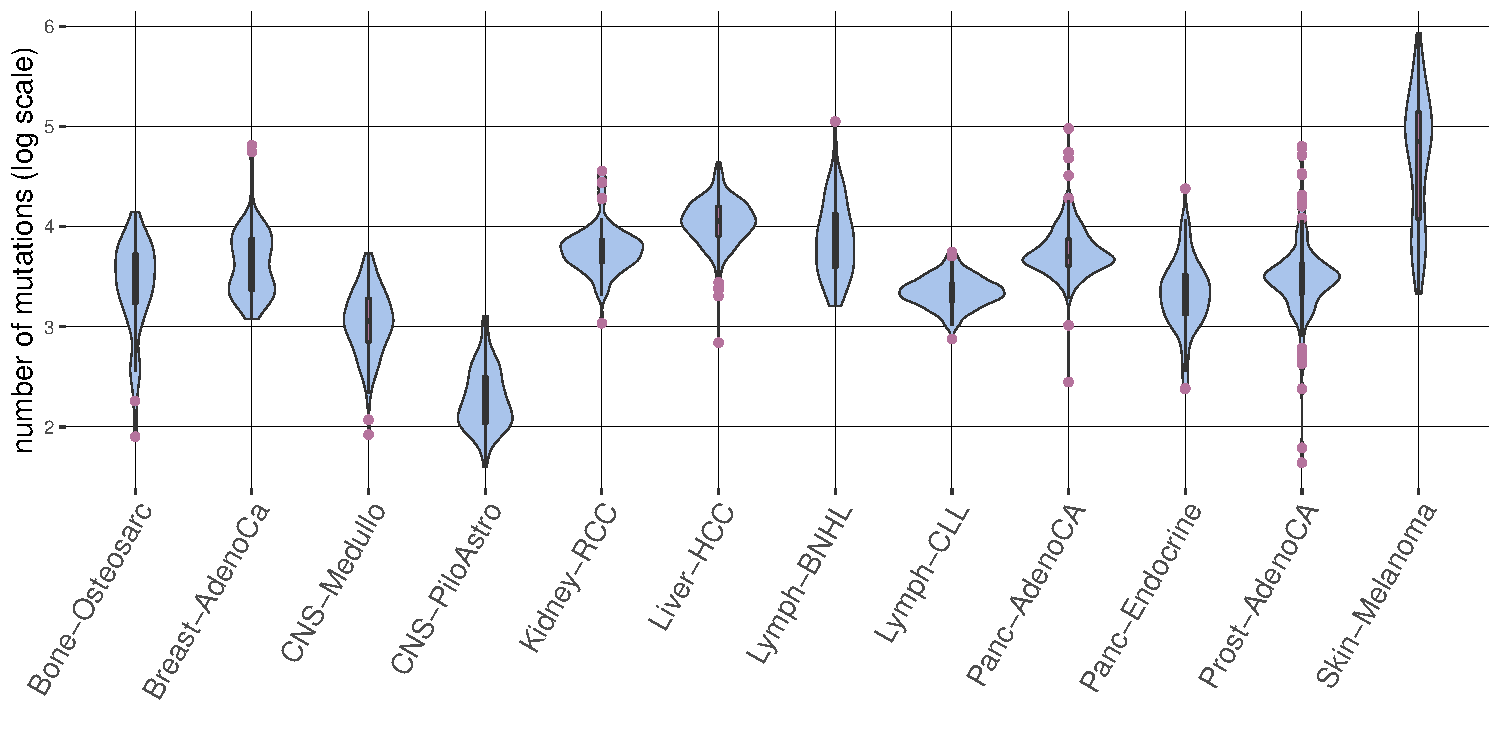
\includegraphics[scale=0.66]{graphics/mutation_summary.pdf}
    \caption{\textbf{Number of mutations (log scale) for each cancer.} Each dot represents a donor. Most patients have approximately 1000-10000 mutations, but there is a great variation.}
    \label{fig:mutation_summary}
\end{figure}


% \newpage
% \section{How cancer original cell types are related by DHS}
% \begin{table}[hp!]
\centering
\caption{\textbf{12 cancers of interest, their abbreviation and their putative original cell types.} The \textbf{Cell line code} column is the code for DHS data of the original cell type, set by the ENCODE project; \textbf{Source} cites the publication that establishes the relationship between the cancer and the original tissue.}
\label{tab:encode_pca}
\begin{tabulary}{\textwidth}{ ll }
\toprule
\textbf{Original cell type} & \bf{Cancer Type}  \\
\toprule
Osteoblast & Osteosarcoma \\

BreastEpi & Breast-AdenoCa \\

Cerebellum &  CNS-Medullo  \\

CereberumAstro & CNS-PiloAstro \\

KidneyREPTEC & Kidney-RCC \\

Hepatocyte & Liver-HCC \\

BCell & Lymph-BNHL \\

BCell & Lymph-CLL \\

PancEpi & Panc-AdenoCa \\

IsletCell & Panc-Endocrine \\

ProstEpi & Prost-AdenoCa \\

Melanocyte & Skin-Melanoma \\
\bottomrule

\end{tabulary}
\end{table}

% . DHS data for these cells is downloaded from either \href{https://genome.ucsc.edu/cgi-bin/hgFileUi?db=hg19&g=wgEncodeOpenChromDnase}{Duke} or \href{https://genome.ucsc.edu/cgi-bin/hgFileUi?db=hg19&g=wgEncodeUwDnase}{UW} project

\newpage
\section{Supplementary computations for smoothing GLE}
\subsection{Gaussian kernel density estimation}

Kernel functions estimate the density of data at a particular location by measuring the distance from that location to all observed data points. To estimate mutation density across the genome, I used the Gaussian kernel, as follows:

\begin{equation}
    K(u) = \frac{1}{2\pi} e^{\frac{-u^2}{2}}
    \label{eq:gaussian}
\end{equation}

where $K$ is the kernel function, $u$ is a variable - \textit{i.e.} $\frac{x-X{i}}{h}$ in equation \ref{eq:density}

\subsection{Bandwidth choice}
The bandwidth $h$ determines the level of smoothing, or the distance at which the an observed mutation can meaningfully influence the density $\hat{f}$ at location $x$, I used the Scott's method, as follows:

\begin{equation}
    h = 1.059 A n^{-1/5}
    \label{eq:bandwidth}
\end{equation}

where $h$ is the bandwidth, $A$ is a measure of spread of the observed mutation locations (\textit{i.e.} the smaller of (1) the standard deviation and the (2) inter-quartile range) and $n$ is the total number of mutations.


\newpage
\section{Supplementary computations for SCE}

\subsection{Deviance residuals for GLM of contingency table}
\begin{equation}
    r_i = sign(y_i - \hat{\mu}_i) \times \sqrt{2y_i\ln{\frac{y_i}{\hat{\mu}_i}} - (y_i - \hat{\mu}_i)}
    \label{eq:dev_res}
\end{equation}
where $r_i$ is the deviance residual for entry $i$, $y_i$ is the actual observed count of that entry, $\hat{\mu}_i$ is the estimated expected count for that entry under the saturated model. The $sign$ function determines the sign of the residual $r_i$, \textit{i.e.} whether it is positive ($>$0) or negative ($<$0). In particular, $r_i>0$ if the observed is greater than the expected and vice versa. 

\subsection{Fisher's method}\label{apdx:fisher}
To aggregate $k$ p-values, we could calculate the Fisher statistic $X$

\begin{equation}
    X = 2 \sum_{i=1}^k \ln{p_i}
    \label{eq:fisher}
\end{equation}
where $X$ is the Fisher statistic, $p_i$ is the member p-value. If converted from the log scale as seen in equation \ref{eq:fisher} to the normal scale, we could see that this is essentially the square of the product of the p-values. $X$ follows the $\chi^2_{2k}$ distribution, so we can easily obtain an aggregated p-value by contrasting $X$ against $\chi^2_{2k}$.

\newpage
\section{Supplementary computations for training classifier}

\subsection{Accuracy measures}

\subsubsection{Sensitivity}
\begin{equation}
    sensitivity_A = \frac{A_{pred(T)}}{A_{true}} 
    \label{eq:sensitivity}
\end{equation}
where $sensitivity_A$ is the sensitivity for identifying A; $A_{pred}$ is the number of A's correctly predicted; $A_{true}$ is the number of true A's

\subsubsection{Specificity}
\begin{equation}
    specificity_A = \frac{A_{pred(T)}}{A_{pred}}
    \label{eq:specificity}
\end{equation}
where $specificity_A$ is the specificity for an observation to be A if it is predicted to be A; $A_{pred(T)}$ is the number of correctly predicted A; $A_{pred}$ is the number of observations predicted to be A.

\subsection{Kullback-Leibler divergence}
The Kullback Leibler divergence of M from P is calculated as follows:

\begin{equation}
    d_{KL}(P|M) = \sum_{x \in X} p(x) \ln{\frac{p(x)}{m(x)}}
    \label{eq:kl}
\end{equation}
where $X$ is the probability space on which $P$ and $M$ are defined; $p$ and $m$ represent the probability of $P$ and $Q$ at $x$.

\subsection{Converting kernel to distance matrix}

\begin{equation}
    d(x,y) = \sqrt{k(x,x) + k(y,y) - 2k(x,y)} 
    \label{eq:k2d_ori}
\end{equation}
where $d(x,y)$ is the entry for $x$ and $y$ to the joint distance matrix; $k(x,y)$ is the entry to the kernel matrix $J$. Because using the Laplacian kernel forces the diagonals, or $k(x,x)$ and $k(y,y)$, to be 1, the formula could be simplified as in \ref{eq:k2d}.

\newpage
\section{Mutation density with respect to chromatin status}

\begin{figure}[h!]
    \begin{subfigure}{.5\textwidth}
    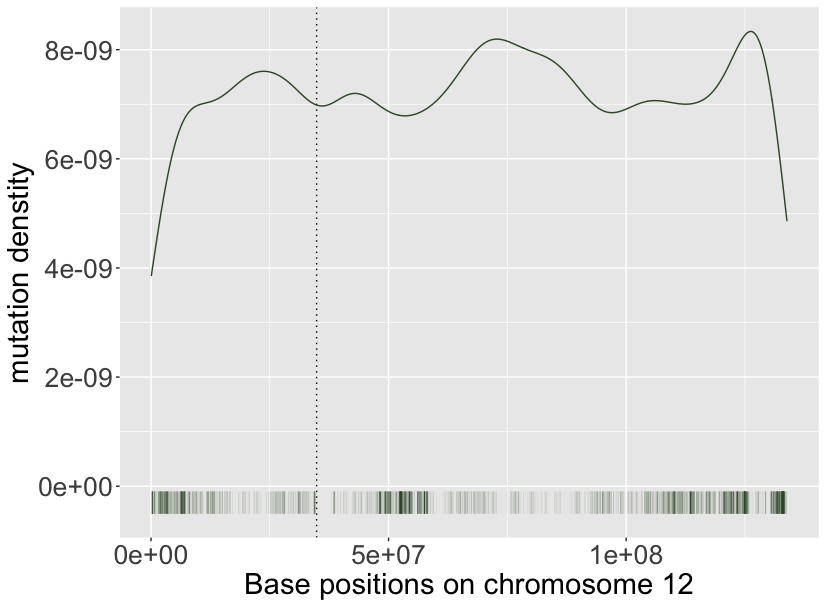
\includegraphics[width=\linewidth,height=0.6\textwidth]{graphics/mutdistribution_Breast-AdenoCa.png}
    \caption{Breast-AdenoCa}
    \end{subfigure}
    ~
    \begin{subfigure}{.5\textwidth}
    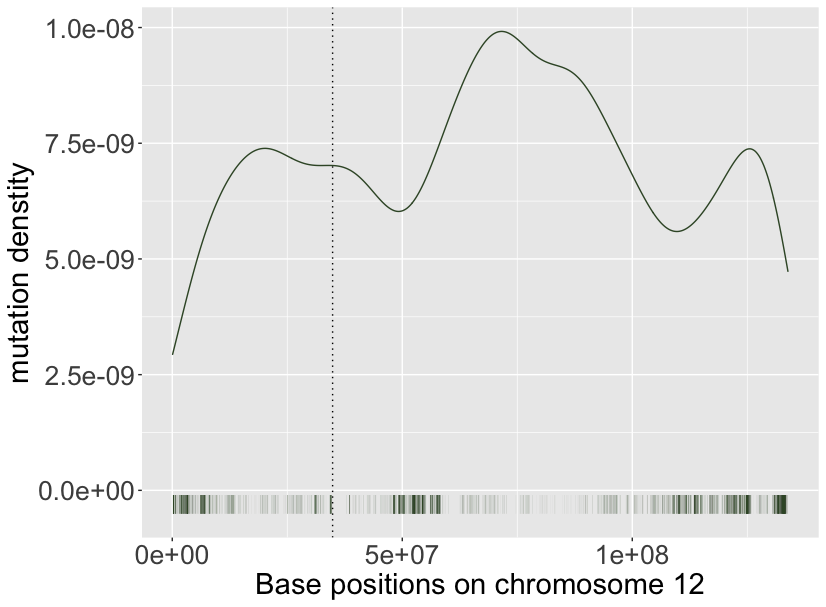
\includegraphics[width=\linewidth,height=0.6\textwidth]{graphics/mutdistribution_Bone-Osteosarc.png}
    \caption{Bone-Osteosarc}
    \end{subfigure} \\
    \vspace{0.2cm}
    
    \begin{subfigure}{.5\textwidth}
    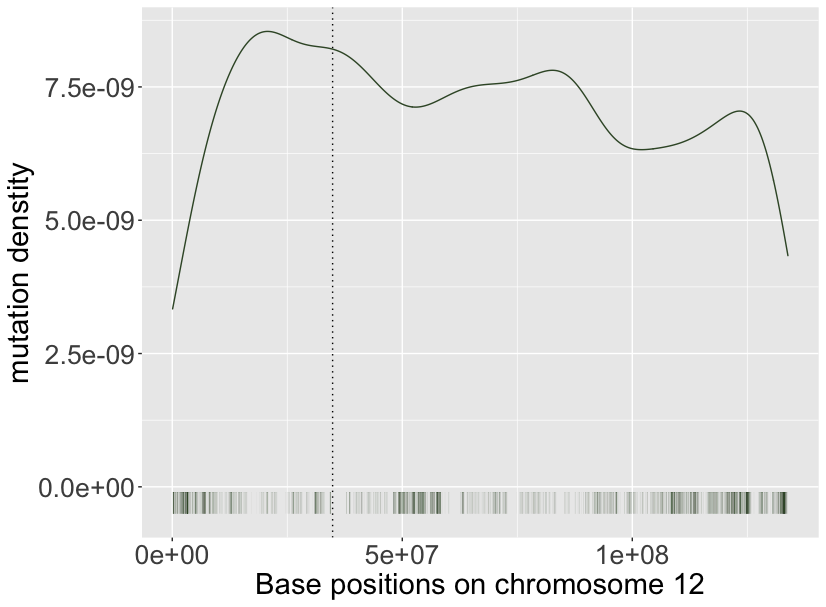
\includegraphics[width=\linewidth,height=0.6\textwidth]{graphics/mutdistribution_CNS-Medullo.png}
    \caption{CNS-Medullo}
    \end{subfigure}
    ~
    \begin{subfigure}{.5\textwidth}
    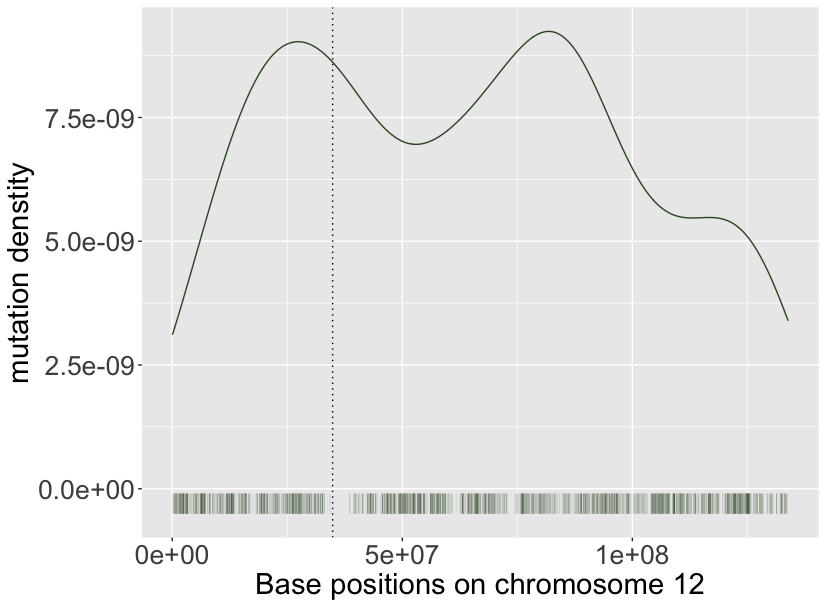
\includegraphics[width=\linewidth,height=0.6\textwidth]{graphics/mutdistribution_CNS-PiloAstro.png}
    \caption{CNS-PiloAstro}
    \end{subfigure} \\
    \vspace{0.2cm}
    
    \begin{subfigure}{.5\textwidth}
    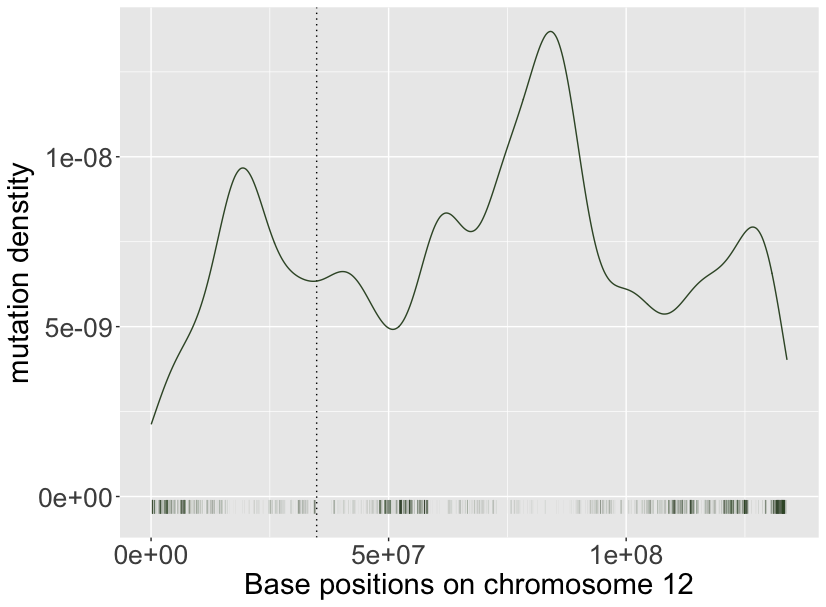
\includegraphics[width=\linewidth,height=0.6\textwidth]{graphics/mutdistribution_Lymph-BNHL.png}
    \caption{Lymph-BNHL}
    \end{subfigure}
    ~
    \begin{subfigure}{.5\textwidth}
    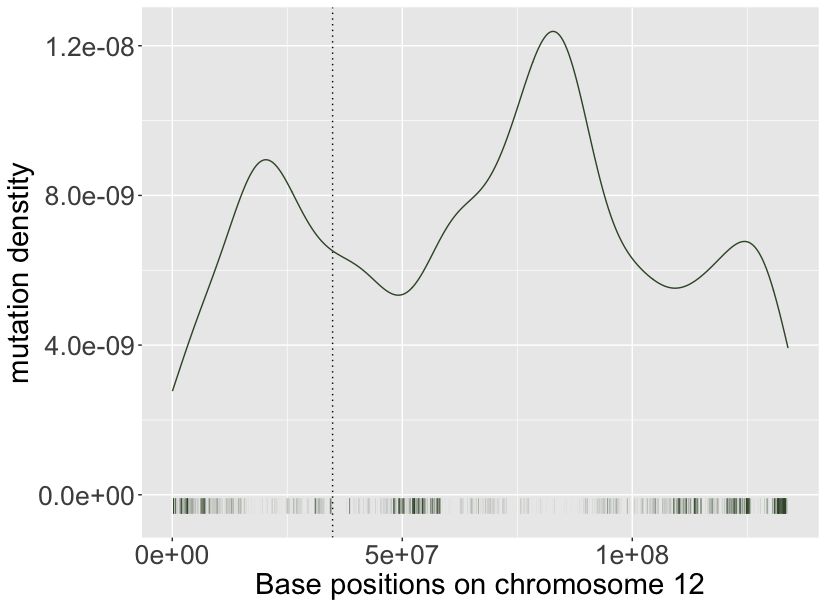
\includegraphics[width=\linewidth,height=0.6\textwidth]{graphics/mutdistribution_Lymph-CLL.png}
    \caption{Lymph-CLL}
    \end{subfigure} \\
    \vspace{0.2cm}
    
    \begin{subfigure}{.5\textwidth}
    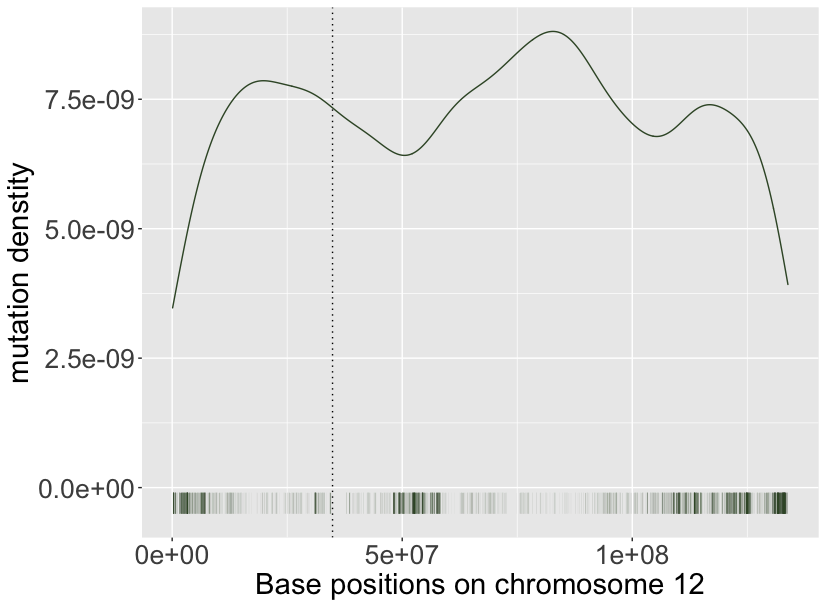
\includegraphics[width=\linewidth,height=0.6\textwidth]{graphics/mutdistribution_Panc-Endocrine.png}
    \caption{Panc-Endocrine}
    \end{subfigure} 
    ~
    \begin{subfigure}{.5\textwidth}
    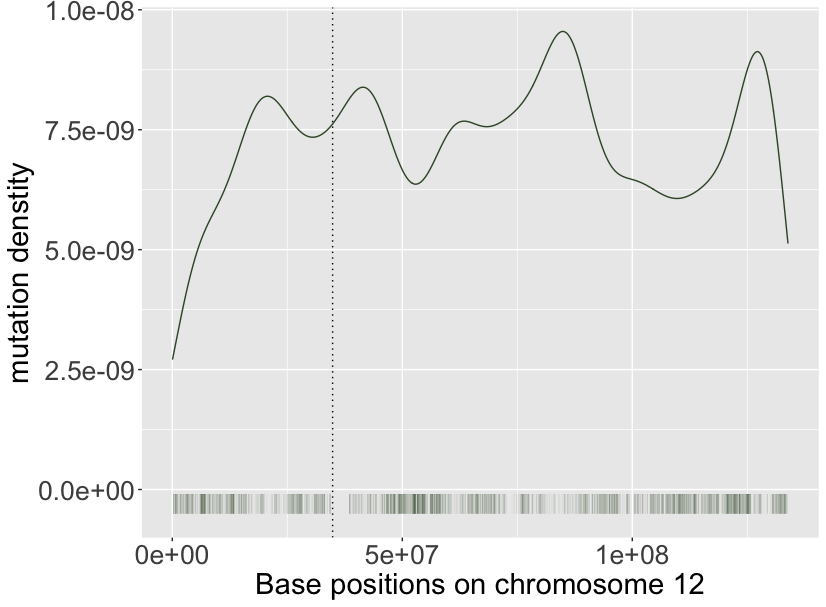
\includegraphics[width=\linewidth,height=0.6\textwidth]{graphics/mutdistribution_Prost-AdenoCA.png}
    \caption{Prost-AdenoCA}
    \end{subfigure} \\

    \caption{\textbf{Mutations tend to be found in closed chromatin regions.} Data for chromosome 12.}
    \label{fig:apdx_mutation_density}
\end{figure}


\newpage
\section{Contingency tables for G-test of independence}\label{apdx:g-test}

\begin{table}[!htb]
    \caption{\textbf{Contingency tables of raw counts for the G-test of independence.} The estimated p-values are reported in Table \ref{tab:g-test}.}
    
    % row 1
    \begin{subtable}[!h]{.5\textwidth}
        \centering
        \begin{tabular}{ l r r }
        \bf{} & \bf{mutated} & \bf{non mutated} \\
        \hline
        closed &  152518 &  2807114120 \\
        open &    3231 &    73763417 \\
        \end{tabular}
        \vspace{0.2cm}
    \subcaption{Bone-Osteosarc}
    \end{subtable} 
    \quad % for side by side tables
    \begin{subtable}[!h]{.5\textwidth}
        \centering
        \begin{tabular}{ l r r }
        \bf{} & \bf{mutated} & \bf{non mutated} \\
        \hline
        closed &  650480 &  2808984887 \\
        open &   17425 &    71380494 \\
        \end{tabular}
        \vspace{0.2cm}
    \subcaption{Breast-AdenoCA}
    \end{subtable}  
    \vspace{0.5cm}
    
    % row 2
    \begin{subtable}[!h]{.5\textwidth}
        \centering
        \begin{tabular}{ l r r }
        \bf{} & \bf{mutated} & \bf{non mutated} \\
        \hline
        closed &  189553 &  2813626572 \\
        open &    3709 &    67213452 \\
        \end{tabular}
        \vspace{0.2cm}
    \subcaption{CNS-Medullo}
    \end{subtable} 
    \quad % for side by side tables
    \begin{subtable}[!h]{.5\textwidth}
        \centering
        \begin{tabular}{ l r r }
        \bf{} & \bf{mutated} & \bf{non mutated} \\
        \hline
        closed &   19922 &  2854648714 \\
        open &     161 &    26364489 \\
        \end{tabular}
        \vspace{0.2cm}
    \subcaption{CNS-PiloAstro}
    \end{subtable}  
    \vspace{0.5cm}
    
    % row 3
    \begin{subtable}[!h]{.5\textwidth}
        \centering
        \begin{tabular}{ l r r }
        \bf{} & \bf{mutated} & \bf{non mutated} \\
        \hline
        closed &  501865 &  2855746381 \\
        open &    4705 &    24780335 \\
        \end{tabular}
        \vspace{0.2cm}
    \subcaption{Kidney-RCC}
    \end{subtable} 
    \quad % for side by side tables
    \begin{subtable}[!h]{.5\textwidth}
        \centering
        \begin{tabular}{ l r r }
        \bf{} & \bf{mutated} & \bf{non mutated} \\
        \hline
        closed & 3102315 &  2772995653 \\
        open &   74679 &   104860639 \\
        \end{tabular}
        \vspace{0.2cm}
    \subcaption{Liver-HCC}
    \end{subtable}  
    \vspace{0.5cm}
    
    % row 4 
    \begin{subtable}[!h]{.5\textwidth}
        \centering
        \begin{tabular}{ l r r }
        \bf{} & \bf{mutated} & \bf{non mutated} \\
        \hline
        closed & 1017447 &  2799576380 \\
        open &   25232 &    80414227 \\
        \end{tabular}
        \vspace{0.2cm}
    \subcaption{Lymph-BNHL}
    \end{subtable} 
    \quad % for side by side tables
    \begin{subtable}[!h]{.5\textwidth}
        \centering
        \begin{tabular}{ l r r }
        \bf{} & \bf{mutated} & \bf{non mutated} \\
        \hline
        closed &  209160 &  2800384667 \\
        open &    4127 &    80435332 \\
        \end{tabular}
        \vspace{0.2cm}
    \subcaption{Lymph-CLL}
    \end{subtable}  
    \vspace{0.5cm}
    
    % row 5
    \begin{subtable}[!h]{.5\textwidth}
        \centering
        \begin{tabular}{ l r r }
        \bf{} & \bf{mutated} & \bf{non mutated} \\
        \hline
        closed & 1548338 &  2829060803 \\
        open &   22149 &    50401996 \\
        \end{tabular}
        \vspace{0.2cm}
    \subcaption{Panc-AdenoCA}
    \end{subtable} 
    \quad % for side by side tables
    \begin{subtable}[!h]{.5\textwidth}
        \centering
        \begin{tabular}{ l r r }
        \bf{} & \bf{mutated} & \bf{non mutated} \\
        \hline
        closed &  239023 &  2812280501 \\
        open &    5613 &    68508149 \\
        \end{tabular}
        \vspace{0.2cm}
    \subcaption{Panc-Endocrine}
    \end{subtable}  
    \vspace{0.5cm}
    
    % row 6
    \begin{subtable}[!h]{.5\textwidth}
        \centering
        \begin{tabular}{ l r r }
        \bf{} & \bf{mutated} & \bf{non mutated} \\
        \hline
        closed &  682486 &  2825381372 \\
        open &   10992 &    54958436 \\
        \end{tabular}
        \vspace{0.2cm}
    \subcaption{Prost-AdenoCA}
    \end{subtable} 
    \quad % for side by side tables
    \begin{subtable}[!h]{.5\textwidth}
        \centering
        \begin{tabular}{ l r r }
        \bf{} & \bf{mutated} & \bf{non mutated} \\
        \hline
        closed & 7128544 &  2830272751 \\
        open &   54685 &    43577306 \\
        \end{tabular}
        \vspace{0.2cm}
    \subcaption{Skin-Melanoma}
    \end{subtable}  
    \label{fig:tab_g-test_contingency}
\end{table}

\newpage
\section{Mislabelled DHS data of chromatin status}
\begin{figure}[h!]
    \centering
    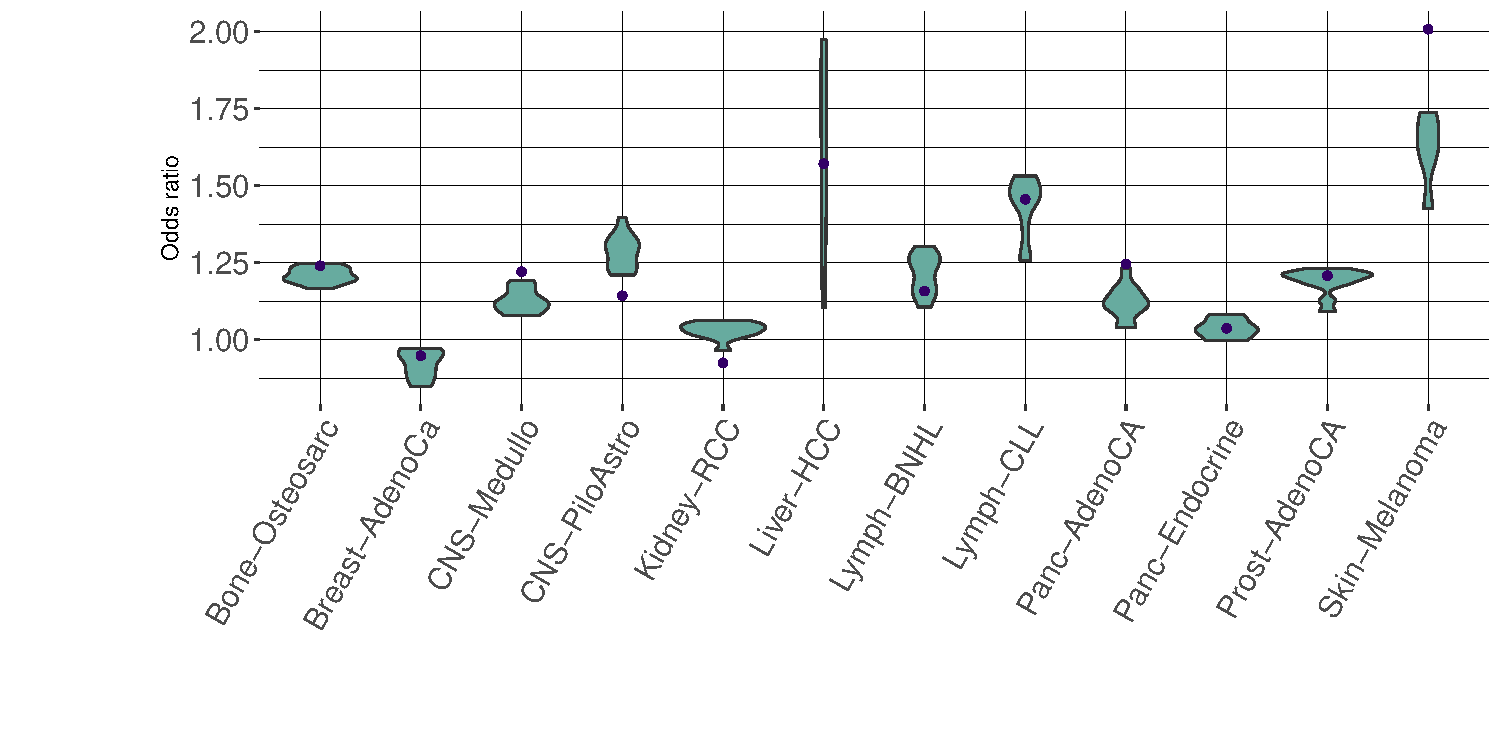
\includegraphics[scale=0.66]{graphics/mixed_or_violin_by_row.pdf}
    \caption{\textbf{Chromatin structure is not discriminative of cancers.} This figure shows an experiment where $OR$'s were calculated by cross-matching DHS data with mutation data of different cancers. The x-axis is the distribution of $OR$ with mislabelled DHS data, the y-axis is the cancers whose mutation data was used, with the purple dot indicating when DHS data of the true cancer was used.}
    \label{fig:mixed_or_byrow}
\end{figure}


\newpage
\section{Base substitutions for individual cancers}
\begin{figure}[ht!]
    \begin{subfigure}{.5\textwidth}
    \centering
    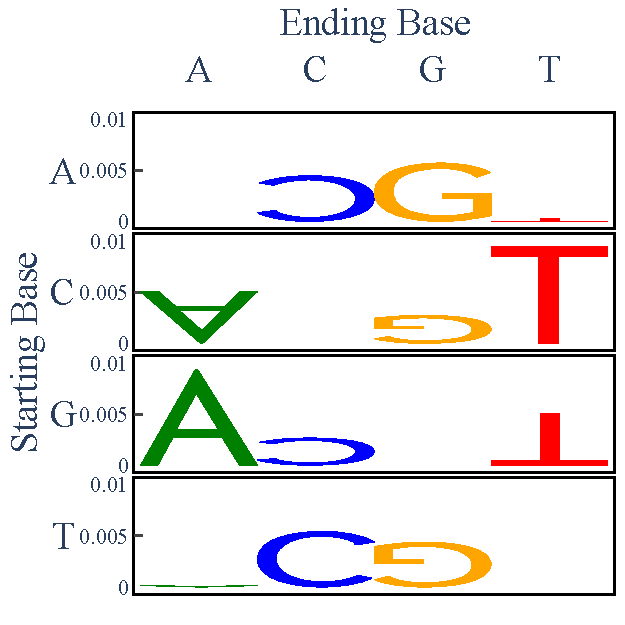
\includegraphics[scale=0.45]{graphics/spectra_Breast-AdenoCa.pdf}
    \caption{Breast-AdenoCa}
    \end{subfigure}
    ~
    \begin{subfigure}{.5\textwidth}
    \centering
    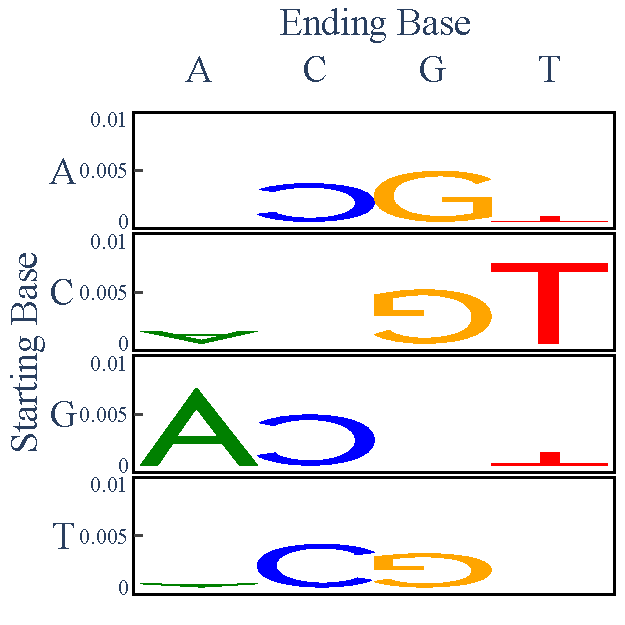
\includegraphics[scale=0.45]{graphics/spectra_Bone-Osteosarc.pdf}
    \caption{Bone-Osteosarc}
    \end{subfigure} \\
    % \vspace{0.1cm}
    
    \begin{subfigure}{.5\textwidth}
    \centering
    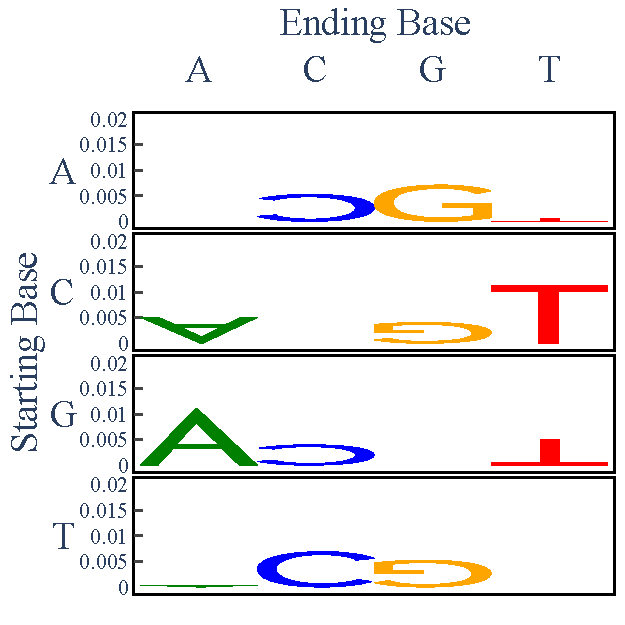
\includegraphics[scale=0.45]{graphics/spectra_CNS-Medullo.pdf}
    \caption{CNS-Medullo}
    \end{subfigure}
    ~
    \begin{subfigure}{.5\textwidth}
    \centering
    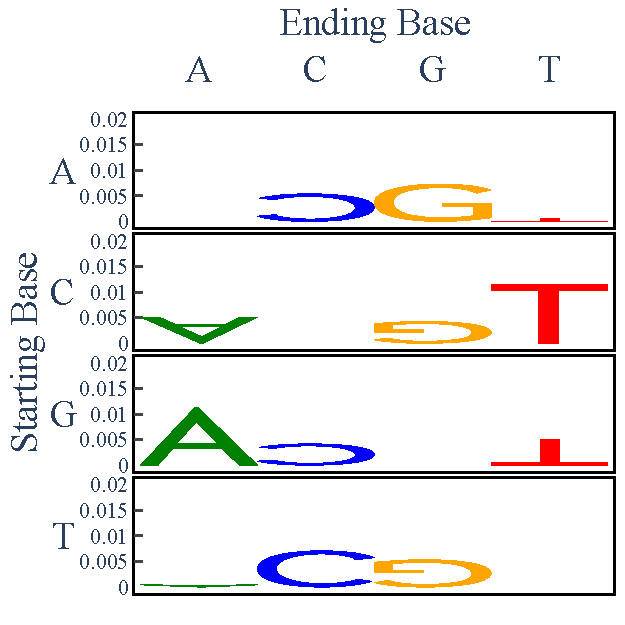
\includegraphics[scale=0.45]{graphics/spectra_CNS-PiloAstro.pdf}
    \caption{CNS-PiloAstro}
    \end{subfigure} \\
    % \vspace{0.1cm}
    
    \begin{subfigure}{.5\textwidth}
    \centering
    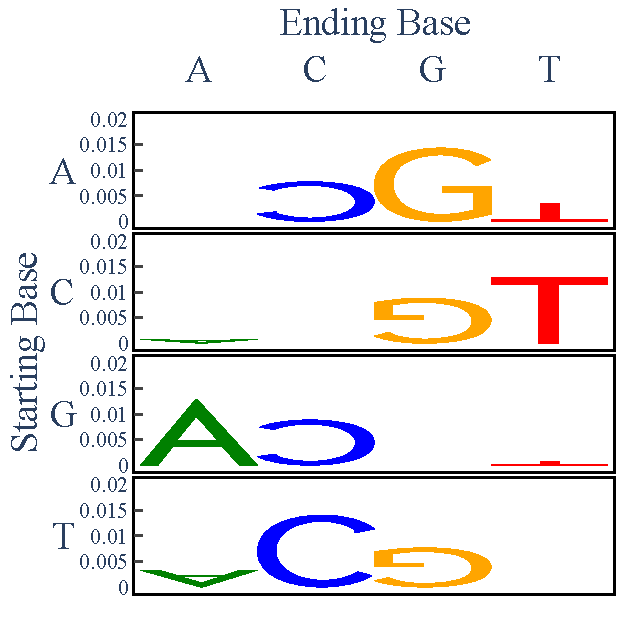
\includegraphics[scale=0.45]{graphics/spectra_Lymph-BNHL.pdf}
    \caption{Lymph-BNHL}
    \end{subfigure}
    ~
    \begin{subfigure}{.5\textwidth}
    \centering
    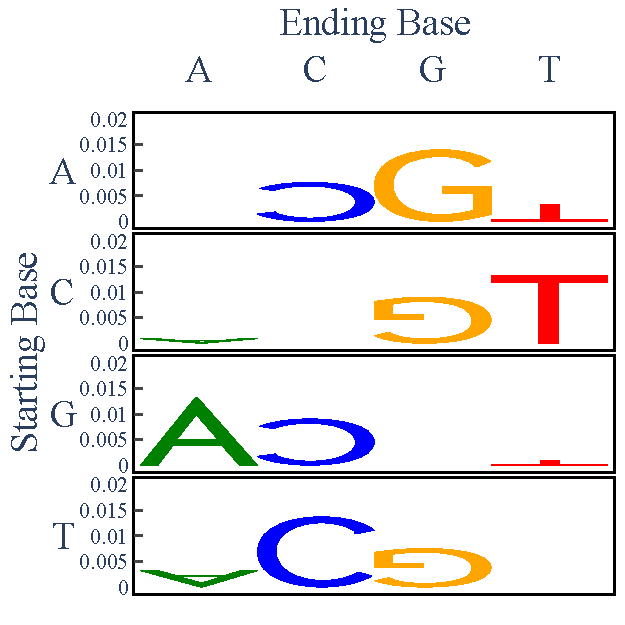
\includegraphics[scale=0.5]{graphics/spectra_Lymph-CLL.pdf}
    \caption{Lymph-CLL}
    \end{subfigure} \\
    % \vspace{0.1cm}
    
    \begin{subfigure}{.5\textwidth}
    \centering
    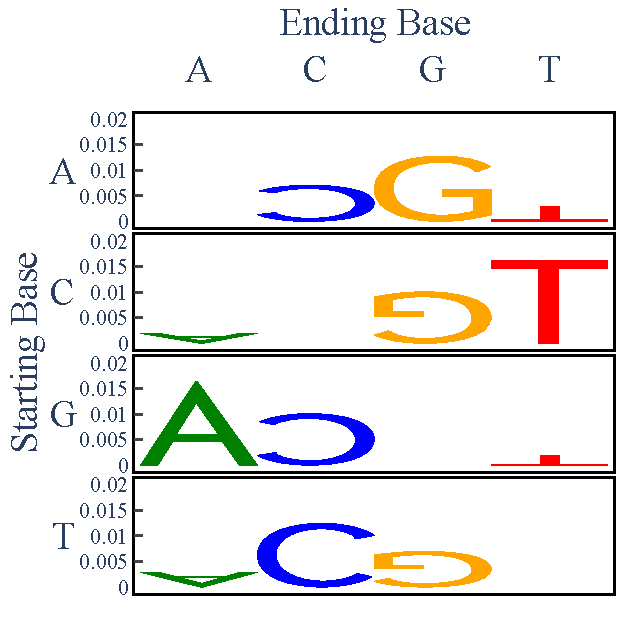
\includegraphics[scale=0.5]{graphics/spectra_Panc-Endocrine.pdf}
    \caption{Panc-Endocrine}
    \end{subfigure} 
    ~
    \begin{subfigure}{.5\textwidth}
    \centering
    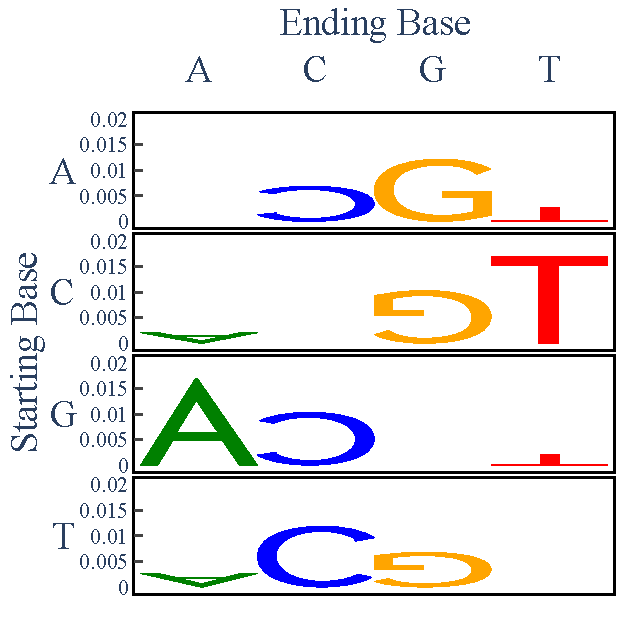
\includegraphics[scale=0.5]{graphics/spectra_Prost-AdenoCA.pdf}
    \caption{Prost-AdenoCA}
    \end{subfigure} \\

    \caption{\textbf{Base substitutions are a rich source of information, manifested by $RE$}}
    \label{fig:apdx_spectra}
\end{figure}


\newpage
\section{Base substitutions when comparing cancers}
\begin{figure}[ht!]
    \begin{subfigure}{.5\textwidth}
    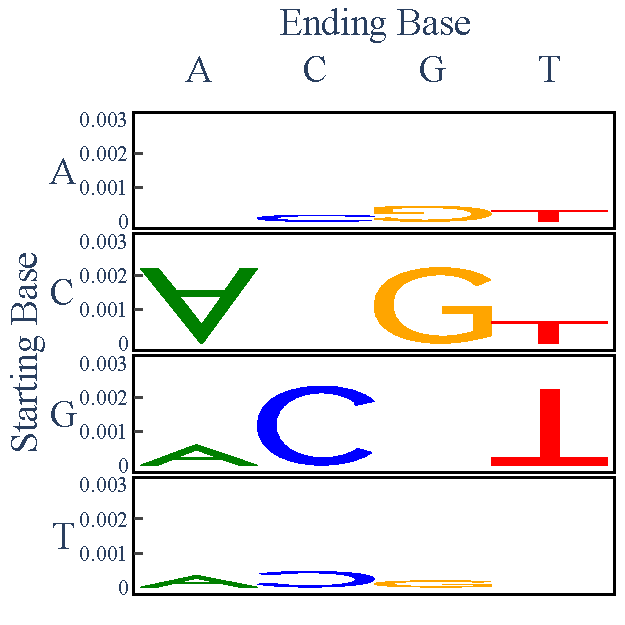
\includegraphics[scale=0.7]{graphics/spectra_CNS-Medullo_Lymph-BNHL.pdf}
    \caption{CNS-Medullo \textit{v.s.} Lymph-BNHL}
    \label{fig:spectra_medullo_bnhl}
    \end{subfigure}
    ~
    \begin{subfigure}{.5\textwidth}
    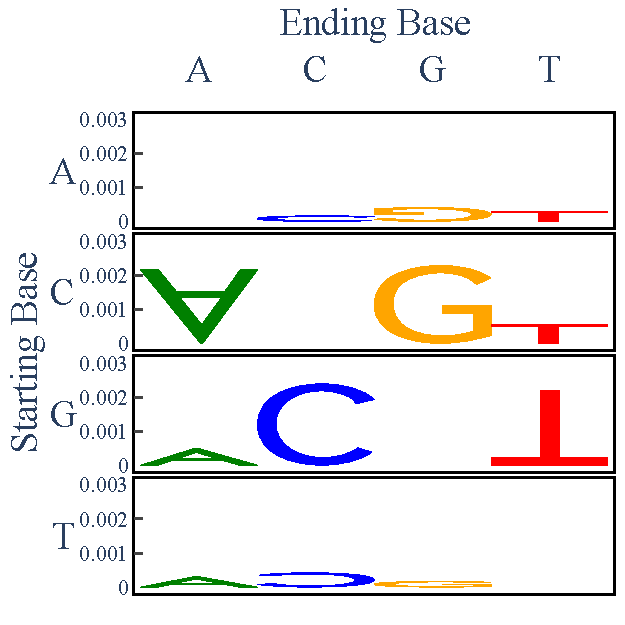
\includegraphics[scale=0.7]{graphics/spectra_CNS-Medullo_Lymph-CLL.pdf}
    \caption{CNS-Medullo \textit{v.s.} Lymph-CLL}
    \label{fig:spectra_medullo_cll}
    \end{subfigure} \\
    \vspace{0.5cm}
    
    \begin{subfigure}{.5\textwidth}
    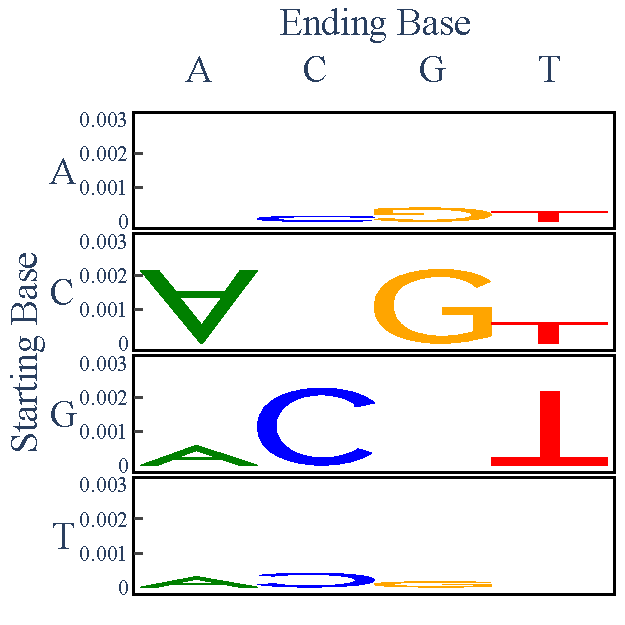
\includegraphics[scale=0.7]{graphics/spectra_CNS-PiloAstro_Lymph-CLL.pdf}
    \caption{CNS-PiloAstro \textit{v.s.} Lymph-CLL}
    \label{fig:spectra_piloastro_cll}
    \end{subfigure}
    ~
    \begin{subfigure}{.5\textwidth}
    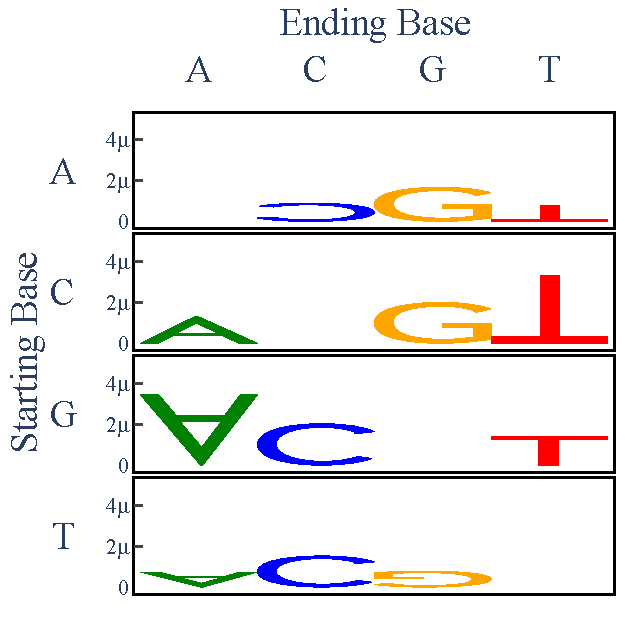
\includegraphics[scale=0.7]{graphics/spectra_Lymph-BNHL_Lymph-CLL.pdf}
    \caption{Lymph-BNHL \textit{v.s.} Lymph-CLL}
    \label{fig:spectra_bnhl_cll}
    \end{subfigure} \\
    \vspace{0.5cm}
    \caption{\textbf{Base substitutions are promising in discriminating cancers according to $RE$ between cancer pairs.} For each panel, each row was derived from a pair of GLMs. The x-axis is the wildtype base; the y-axis is the product of the substitution. The heights of the letters are $RE$'s. An up-orientation indicates an excess while a down-orientation indicates a deficit of the mutation when comparing the (a) CNS-Medullo to Lymph-BNHL, (b) CNS-Medullo to Lymph-CLL, (c) CNS-PiloAstro to Lymph-CLL, (d) Lymph-BNHL to Lymph-CLL. This is an extension of Figure \ref{fig:paired_spectra} in the main text.}
    \label{fig:apdx_paired_spectra}
\end{figure}

\newpage
\section{Supplementary confusion matrices}



